\documentclass[CJK,utf8]{ctexrep}

\usepackage{tabularx}
\usepackage{listings}
\usepackage{multirow}
\usepackage{amsmath}

%加工描述语言
\lstdefinestyle{proc}{
	basicstyle=\footnotesize\ttfamily,
	keywordstyle=\bfseries,
	keepspaces=true,
	showspaces=false,
	language=[Visual]Basic,	%覆盖了绝大多数需要的关键字
	%这里加额外需要的关键字
	otherkeywords={SWITCH, GENERATE, BASED, TO},
	%这里删除原有的关键字,虽然不应该有?
	deletekeywords={}
}

% Title Page
\title{
	考试招生录取系统\\
	\large 需求分析与结构化设计文档
}
\author{
	\begin{tabular}{ll}
		12307130129 & 刘宇达 \\
		11307120059 & 王家威 \\
		12307130222 & 李砚业 \\
		11307110008 & 甘全 \\
	\end{tabular}
}


\begin{document}
\maketitle

\section*{引言}

\subsection*{系统概述}
考试招生录取系统通过信息化的方式涵盖了招生录取管理系统填报志愿、招生、投档等
环节,提供了如下功能:
\begin{enumerate}
	\item 院校招生计划管理及发布
	\item 成绩管理及发布
	\item 志愿填报管理
	\item 调档分数线的划定
	\item 招生过程的维护,包括统招、调招、特招、退档、补录等
	\item 录取名册及各个考生录取信息的发布
\end{enumerate}

%直接抄了。。
系统流程以数据流图的方式展现,并辅以数据字典对数据流图中的所有名词加以解释。
与此同时,数据字典中规定了所有数据流的组成项,每个数据项规定了相应的取值类型和范围,
使系统不易出错、可靠性高;而加工图进一步描述了数据流的变化过程,简明易懂。
最后,通过结构图展现了系统由哪些模块组成,以及模块之间的调用关系,
使整套系统的构建更为清晰。

\subsection*{文档概述}
%继续抄。。
本文档详细描述了考试招生录取系统的需求规约,为进一步设计及具体实现奠定了基础。
%参考文献就不要了吧

\section*{项目概述}

\subsection*{目标}
%其实就是变换了一下需求的用语。。
将信息化应用于考试招生录取系统中,方便统一协调考生、招生办、院校之间的关系,提高
办公效率。

\subsection*{用户特点}
本系统由于面向考生、招生办及院校,对考生将来人生规划及发展,以及院校生源的质量把关
有重要影响,
%继续堂而皇之地抄。。
因此要求可靠性较高。对于各类关键数据,设置权限,保证不会被恶意修改。
此外,各项功能差别较大,各模块所需要的操作各不相同,需要分别进行针对性的开发,
才能更好地利用资源。

\section*{需求规定}

考试招生录取系统分为两大模块:\emph{报名模块}及\emph{招生模块}。
其还需要两个数据库,分别保存\emph{考生档案}及\emph{审核后的招生信息}。
以下文档中的\emph{招生信息},若无特殊说明,均指审核后的招生信息。

\subsection*{报名模块}

考生在报名志愿之前,需要查询各个院校的招生信息,包括招生要求、学费等,
以帮助其选择理想的院校。因此,报名模块需要从招生信息数据库中,
读取考生需要查看院校的招生信息,并反馈给考生。

随后,考生需要填写考生基本信息,以及其希望的志愿。报名模块收集这些信息,
在检查后存入考生档案数据库中。

考试结束之后,招生办需要往各个考生的档案中录入其成绩,包括各科成绩以及总成绩。
报名模块亦需要接收成绩信息,并依此更新考生档案数据库。

\subsection*{招生模块}

招生分为三个步骤:审核、投档和录取。因此,招生模块分为如下三个子模块:

\begin{enumerate}
	\item 审核子模块
	
	审核子模块用以接收各院校的招生信息,审核这些信息并发送审核结果,
	以及向考生展示审核后的招生信息。审核通过后的招生信息被存入招生信息数据库中。
	
	\item 投档子模块
	
	系统从招生信息数据库中读取各个学校的录取批次、计划招生数据、调档比例等,
	并获取统计各个考生的成绩,计算各学校的调档分数线。
	如果调档比例为100\%,则说明不扩大范围调档。在调档时如果最后几位分数相同,
	如果不调它,又不足计划数,调它又超过计划数,系统自动保持其调档。
	
	投档子模块计算得到的各个学校计划招生数与其余信息一起被传递到录取子模块中。
	
	\item 录取子模块
	
	录取子模块最为复杂,需要维护每个考生的状态(录取、退档、特招、补录),
	进行统招、调招、特招、补录、退档等工作,并负责展示录取结果。
	这些都需要各自的部件来完成。
\end{enumerate}

\section*{系统设计}

\subsection*{数据流图}

\begin{enumerate}
	\item 顶层图
	
	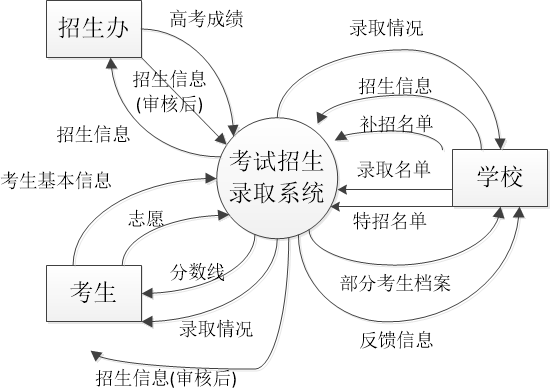
\includegraphics[scale=0.75]{DataFlowDiagram/顶层图.png}
	
	\item 0层图
	
	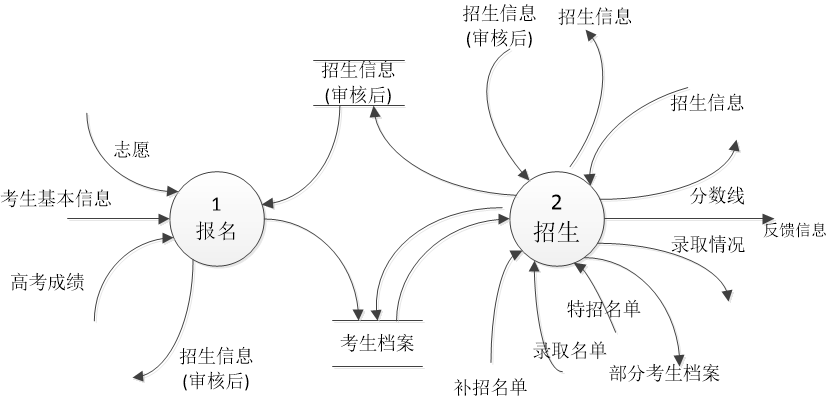
\includegraphics[scale=0.5]{DataFlowDiagram/0层图.png}
	
	\item 加工2(招生模块)子图
	
	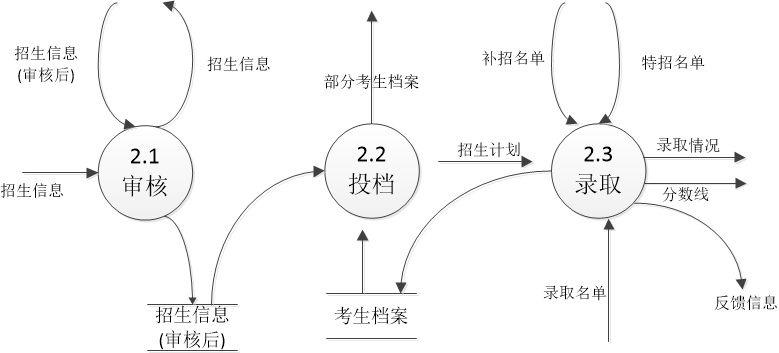
\includegraphics[scale=0.55]{DataFlowDiagram/加工2子图.png}
	
	\item 加工2.3(录取子模块)子图
	
	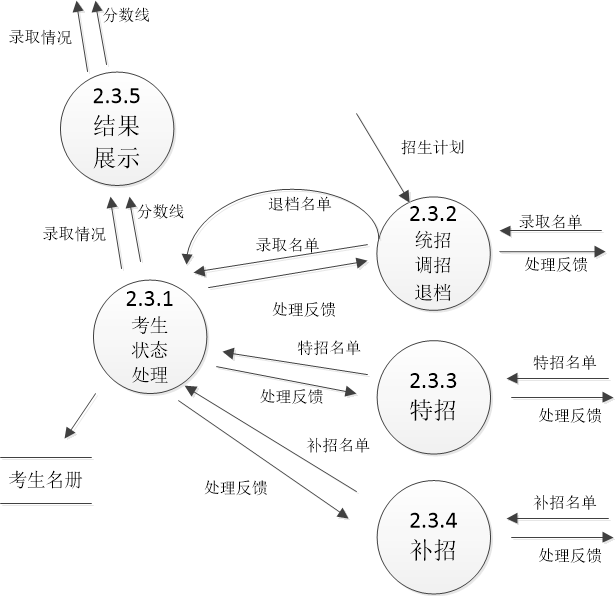
\includegraphics[scale=0.65]{DataFlowDiagram/加工2.3子图.png}
\end{enumerate}

\subsection*{数据字典}

%
% 表格示例:
%

\subsubsection*{数据项条目}

\begin{tabularx}{0.85\textwidth}{|l|X|}
	\hline
	\textbf{名称} & \textbf{考生号} \\
	\hline
	简述 & 考生唯一识别号 \\
	\hline
	数据类型 & 11位数字字符串 \\
	\hline
	\multirow{4}{*}{备注}
	& 1-2位:地区代码 \\
	& 3-4位:城市代码 \\
	& 5-7位:学校代码 \\
	& 8-11位:唯一编号 \\
	\hline
\end{tabularx}

\begin{tabularx}{0.85\textwidth}{|l|X|}
	\hline
	\textbf{名称} & \textbf{姓名} \\
	\hline
	简述 & 考生姓名 \\
	\hline
	数据类型 & 字符串 \\
	\hline
\end{tabularx}

\begin{tabularx}{0.85\textwidth}{|l|X|}
	\hline
	\textbf{名称} & \textbf{毕业院校} \\
	\hline
	简述 & 考生毕业院校 \\
	\hline
	数据类型 & 字符串 \\
	\hline
	取值范围 & 省内高中 \\
	\hline
	备注 & 从下拉式菜单中选择 \\
	\hline
\end{tabularx}

\begin{tabularx}{0.85\textwidth}{|l|X|}
	\hline
	\textbf{名称} & \textbf{毕业年份} \\
	\hline
	简述 & 考生毕业年份 \\
	\hline
	数据类型 & 4位整型 \\
	\hline
	取值范围 & 2000...2999 \\
	\hline
\end{tabularx}

\begin{tabularx}{0.85\textwidth}{|l|X|}
	\hline
	\textbf{名称} & \textbf{通信地址} \\
	\hline
	简述 & 考生通信地址 \\
	\hline
	数据类型 & 字符串 \\
	\hline
	备注 & 用于录取通知书寄送 \\
	\hline
\end{tabularx}

\begin{tabularx}{0.85\textwidth}{|l|X|}
	\hline
	\textbf{名称} & \textbf{联系电话} \\
	\hline
	简述 & 考生联系电话 \\
	\hline
	数据类型 & 11位数字字符串 \\
	\hline
	备注 & 固定电话应包含区号 \\
	\hline
\end{tabularx}

\begin{tabularx}{0.85\textwidth}{|l|X|}
	\hline
	\textbf{名称} & \textbf{语文成绩} \\
	\hline
	简述 & 考生语文成绩 \\
	\hline
	数据类型 & 整型 \\
	\hline
	取值范围 & 0...150 \\
	\hline
\end{tabularx}

\begin{tabularx}{0.85\textwidth}{|l|X|}
	\hline
	\textbf{名称} & \textbf{数学成绩} \\
	\hline
	简述 & 考生数学成绩 \\
	\hline
	数据类型 & 整型 \\
	\hline
	取值范围 & 0...150 \\
	\hline
\end{tabularx}

\begin{tabularx}{0.85\textwidth}{|l|X|}
	\hline
	\textbf{名称} & \textbf{英语成绩} \\
	\hline
	简述 & 考生英语成绩 \\
	\hline
	数据类型 & 整型 \\
	\hline
	取值范围 & 0...150 \\
	\hline
\end{tabularx}

\begin{tabularx}{0.85\textwidth}{|l|X|}
	\hline
	\textbf{名称} & \textbf{综合科成绩} \\
	\hline
	简述 & 考生综合科成绩 \\
	\hline
	数据类型 & 整型 \\
	\hline
	取值范围 & 0...300 \\
	\hline
\end{tabularx}

\begin{tabularx}{0.85\textwidth}{|l|X|}
	\hline
	\textbf{名称} & \textbf{总成绩} \\
	\hline
	简述 & 考生总成绩 \\
	\hline
	数据类型 & 整型 \\
	\hline
	取值范围 & 0...750 \\
	\hline
	\multirow{2}{*}{备注} & $\text{总成绩}=\text{语文成绩}+\text{数学成绩}
	+\text{英语成绩}+\text{综合科成绩}$ \\
	\hline
\end{tabularx}

\begin{tabularx}{0.85\textwidth}{|l|X|}
	\hline
	\textbf{名称} & \textbf{排名} \\
	\hline
	简述 & 考生排名 \\
	\hline
	数据类型 & 整型 \\
	\hline
	取值范围 & $1\le \text{排名} \le \text{考生总人数}$\\
	\hline
	备注 & 根据排名规则产生 \\
	\hline
\end{tabularx}

\begin{tabularx}{0.85\textwidth}{|l|X|}
	\hline
	\textbf{名称} & \textbf{志愿院校专业} \\
	\hline
	简述 & 考生志愿院校专业 \\
	\hline
	数据类型 & 字符串 \\
	\hline
	取值范围 & 可填报院校和专业 \\
	\hline
\end{tabularx}

\begin{tabularx}{0.85\textwidth}{|l|X|}
	\hline
	\textbf{名称} & \textbf{录取状态} \\
	\hline
	简述 & 考生录取状态 \\
	\hline
	\multirow{2}{*}{数据类型} & 自定义结构:\\
	& $\lbrace\text{已投档}\vert\text{已录取}\vert\text{未录取}
	\rbrace+\text{志愿院校专业}$ \\
	\hline
\end{tabularx}

\begin{tabularx}{0.85\textwidth}{|l|X|}
	\hline
	\textbf{名称} & \textbf{招生人数} \\
	\hline
	简述 & 志愿院校和专业的最大录取人数 \\
	\hline
	数据类型 & 正整型 \\
	\hline
\end{tabularx}

\begin{tabularx}{0.85\textwidth}{|l|X|}
	\hline
	\textbf{名称} & \textbf{招生要求} \\
	\hline
	简述 & 志愿院校和专业的招生要求 \\
	\hline
	数据类型 & 字符串 \\
	\hline
\end{tabularx}

\begin{tabularx}{0.85\textwidth}{|l|X|}
	\hline
	\textbf{名称} & \textbf{院校基本信息} \\
	\hline
	简述 & 志愿院校的基本信息 \\
	\hline
	数据类型 & 字符串 \\
	\hline
\end{tabularx}

\begin{tabularx}{0.85\textwidth}{|l|X|}
	\hline
	\textbf{名称} & \textbf{录取批次} \\
	\hline
	简述 & 志愿院校的录取批次\\
	\hline
	数据类型 & 字符串 \\
	\hline
	取值范围 & $\lbrace\text{提前批次}\vert\text{第一批次}\vert
	\text{第二批次}\rbrace$ \\
	\hline
\end{tabularx}

\begin{tabularx}{0.85\textwidth}{|l|X|}
	\hline
	\textbf{名称} & \textbf{退档理由} \\
	\hline
	简述 & 给考生的退档理由 \\
	\hline
	数据类型 & 字符串 \\
	\hline
\end{tabularx}

\begin{tabularx}{0.85\textwidth}{|l|X|}
	\hline
	\textbf{名称} & \textbf{特招说明} \\
	\hline
	简述 & 特招考生的说明 \\
	\hline
	数据类型 & 字符串 \\
	\hline
\end{tabularx}

\begin{tabularx}{0.85\textwidth}{|l|X|}
	\hline
	\textbf{名称} & \textbf{补招说明} \\
	\hline
	简述 & 补招考生的说明 \\
	\hline
	数据类型 & 字符串 \\
	\hline
\end{tabularx}

\begin{tabularx}{0.85\textwidth}{|l|X|}
	\hline
	\textbf{名称} & \textbf{反馈信息} \\
	\hline
	简述 & 招生办对录取情况的反馈信息 \\
	\hline
	数据类型 & 字符串 \\
	\hline
\end{tabularx}

\subsubsection*{数据流条目}

\begin{tabularx}{0.85\textwidth}{|l|X|}
	\hline
	\textbf{名称} & \textbf{考生基本信息} \\
	\hline
	简述 & 记录考生个人信息 \\
	\hline
	\multirow{2}{*}{组成} & $\text{考生号}+\text{姓名}+\text{毕业院校}
	+\text{毕业年份}+\text{通信地址}+\text{联系电话}$ \\
	\hline
	来源 & 考生 \\
	\hline
	去向 & 报名模块 \\
	\hline
\end{tabularx}

\begin{tabularx}{0.85\textwidth}{|l|X|}
	\hline
	\textbf{名称} & \textbf{高考成绩} \\
	\hline
	简述 & 记录考生高考成绩以及排名 \\
	\hline
	\multirow{2}{*}{组成} & $\text{语文成绩}+\text{数学成绩}
	+\text{英语成绩}+\text{综合科成绩}+\text{总成绩}+\text{排名}$ \\
	\hline
	来源 & 招生办 \\
	\hline
	去向 & 报名模块 \\
	\hline
\end{tabularx}

\begin{tabularx}{0.85\textwidth}{|l|X|}
	\hline
	\textbf{名称} & \textbf{志愿} \\
	\hline
	简述 & 记录考生各志愿情况 \\
	\hline
	组成 & $
	\lbrace\text{(一本)志愿院校专业}\rbrace_1^4
	+\lbrace\text{(二本)志愿院校专业}\rbrace_1^4$ \\
	\hline
	来源 & 考生 \\
	\hline
	去向 & 报名模块 \\
	\hline
	\multirow{2}{*}{备注} & 
	考生可根据情况在每批次院校中填报四所志愿学校作为平行志愿 \\
	\hline
\end{tabularx}

\begin{tabularx}{0.85\textwidth}{|l|X|}
	\hline
	\textbf{名称} & \textbf{考生档案} \\
	\hline
	\multirow{2}{*}{简述} & 
	报名处理模块根据考生基本信息、志愿信息和高考成绩生成的考生档案 \\
	\hline
	组成 & $\lbrace
	\text{考生基本信息}+\text{高考成绩}+\text{志愿}+\text{录取状态}
	\rbrace$ \\
	\hline
	来源 & 考生 \\
	\hline
	去向 & 报名模块 \\
	\hline
	备注 & 录取状态一栏在生成考生档案时均为“未录取”状态 \\
	\hline
\end{tabularx}

\begin{tabularx}{0.85\textwidth}{|l|X|}
	\hline
	\textbf{名称} & \textbf{招生计划} \\
	\hline
	简述 & 指定专业的招生的招生人数和招生要求 \\
	\hline
	组成 & $\text{志愿院校专业}+\text{招生人数}+\text{招生要求}$ \\
	\hline
	备注 & 为完整招生信息的一部分 \\
	\hline
\end{tabularx}

\begin{tabularx}{0.85\textwidth}{|l|X|}
	\hline
	\textbf{名称} & \textbf{招生信息} \\
	\hline
	\multirow{2}{*}{简述} & 
	包含学校信息和计划信息,院校发布的招生信息需要招生办审核后生效 \\
	\hline
	组成 & $\text{院校基本信息}+\text{录取批次}+\lbrace
	\text{招生计划}
	\rbrace$ \\
	\hline
	来源 & 1. 院校;2. 招生办 \\
	\hline
	去向 & 1. 招生办;2. 院校、考生、招生信息文件 \\
	\hline
	备注 & 1为审核过程,2为审核后发布过程 \\
	\hline
\end{tabularx}

\begin{tabularx}{0.85\textwidth}{|l|X|}
	\hline
	\textbf{名称} & \textbf{录取情况} \\
	\hline
	简述 & 记录一位考生的录取情况 \\
	\hline
	组成 & $\text{考生基本信息}+\text{志愿院校专业}$ \\
	\hline
	备注 & 为录取、特招、补招名单的条目 \\
	\hline
\end{tabularx}

\begin{tabularx}{0.85\textwidth}{|l|X|}
	\hline
	\textbf{名称} & \textbf{录取名单} \\
	\hline
	简述 & 院校统招和调招的录取名单 \\
	\hline
	组成 & $\lbrace\text{录取情况}\rbrace$ \\
	\hline
	来源 & 院校 \\
	\hline
	去向 & 招生模块 \\
	\hline
	备注 & 需要审核 \\
	\hline
\end{tabularx}

\begin{tabularx}{0.85\textwidth}{|l|X|}
	\hline
	\textbf{名称} & \textbf{退档名单} \\
	\hline
	简述 & 未被录取的考生名单 \\
	\hline
	组成 & $\lbrace\text{考生档案}+\text{退档理由}\rbrace$ \\
	\hline
	来源 & 院校 \\
	\hline
	去向 & 招生模块 \\
	\hline
	备注 & 可为空 \\
	\hline
\end{tabularx}

\begin{tabularx}{0.85\textwidth}{|l|X|}
	\hline
	\textbf{名称} & \textbf{特招名单} \\
	\hline
	简述 & 院校特招的录取名单 \\
	\hline
	组成 & $\lbrace\text{录取情况}+\text{特招说明}\rbrace$ \\
	\hline
	来源 & 院校 \\
	\hline
	去向 & 招生模块 \\
	\hline
	备注 & 院校特长生、议价生的录取,名单需要审核 \\
	\hline
\end{tabularx}

\begin{tabularx}{0.85\textwidth}{|l|X|}
	\hline
	\textbf{名称} & \textbf{补招名单} \\
	\hline
	简述 & 院校补招的录取名单 \\
	\hline
	组成 & $\lbrace\text{录取情况}+\text{补招说明}\rbrace$ \\
	\hline
	来源 & 院校 \\
	\hline
	去向 & 招生模块 \\
	\hline
	备注 & 录取工作结束后,院校进行进行补录,名单需要审核 \\
	\hline
\end{tabularx}

\begin{tabularx}{0.85\textwidth}{|l|X|}
	\hline
	\textbf{名称} & \textbf{反馈信息} \\
	\hline
	简述 & 记录对一位考生录取情况的反馈信息 \\
	\hline
	组成 & $\text{考生基本信息}+\text{反馈描述}$ \\
	\hline
	\multirow{2}{*}{备注} & 反馈描述可能是对不规范的录取进行修改或者警告,
	反馈信息是处理反馈列表的一个条目 \\
	\hline
\end{tabularx}

\begin{tabularx}{0.85\textwidth}{|l|X|}
	\hline
	\textbf{名称} & \textbf{处理反馈} \\
	\hline
	简述 & 招生办对院校录取情况的处理反馈 \\
	\hline
	组成 & $\lbrace\text{反馈信息}\rbrace$ \\
	\hline
	来源 & 招生模块 \\
	\hline
	去向 & 院校 \\
	\hline
	备注 & 处理反馈仅对不规范的录取进行反馈 \\
	\hline
\end{tabularx}

\begin{tabularx}{0.85\textwidth}{|l|X|}
	\hline
	\textbf{名称} & \textbf{分数线} \\
	\hline
	简述 & 某批次或某专业的录取分数线 \\
	\hline
	组成 & $\lbrace\text{志愿院校专业}+\text{录取分数}\rbrace$ \\
	\hline
	来源 & 招生模块 \\
	\hline
	去向 & 院校、考生 \\
	\hline
\end{tabularx}

\subsubsection*{文件条目}

\subsubsection*{加工条目}

\subsubsection*{加工说明}

% 示例加工说明伪代码。
% 如果需要添加关键字可以在开头的\lstdefinestyle那里添加。
Ea.b
\begin{lstlisting}[style=proc]
	GET 考生基本信息
	WRITE TO 考生档案
\end{lstlisting}

\section*{结构设计图}

\end{document}          
